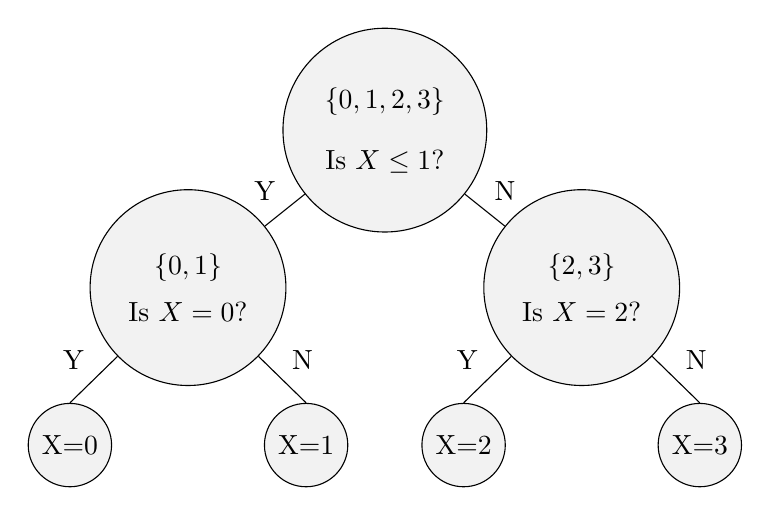
\begin{tikzpicture}[
  decision node/.style={draw, circle, minimum size=1cm, fill=gray!10},
  leaf node/.style={draw, circle, minimum size=1cm, fill=gray!10},
  level distance=1.5cm,
  level 1/.style={sibling distance=4cm},
  level 2/.style={sibling distance=2cm}
]
  % Root node
  % \node[decision node] (root) at (0, 0) {$\{1, 2, 3, 4\}$};
  \node[decision node] (root) at (0, 0) {%
    \parbox{2cm}{\centering $\{0, 1, 2, 3\}$ \\ \vspace{1em} \red{Is $X \leq 1$?}}
  };

  
  % Left child of the root
  \node[decision node] (left) at (-2.5, -2) {%
    \parbox{2cm}{\centering $\{0, 1\}$ \\ \vspace{0.5em} \red{Is $X=0$?}}
  };
  % Right child of the root
  \node[decision node] (right) at (2.5, -2) {%
    \parbox{2cm}{\centering $\{2, 3\}$ \\ \vspace{0.5em} \red{Is $X=2$?}}
  }; 
  % Leaves
  \node[leaf node] (x1) at (-4, -4) {X=0};
  \node[leaf node] (x2) at (-1, -4) {X=1};
  \node[leaf node] (x3) at (1, -4) {X=2};
  \node[leaf node] (x4) at (4, -4) {X=3};
  
  % Edges
  \draw (root) -- node[above left] {Y} (left);
  \draw (root) -- node[above right] {N} (right);
  
  % Edges from the left child
  \draw (left) -- node[above left] {Y} (x1.north);
  \draw (left) -- node[above right] {N} (x2.north);
  
  % Edges from the right child
  \draw (right) -- node[above left] {Y} (x3.north);
  \draw (right) -- node[above right] {N} (x4.north);
\end{tikzpicture}
